\documentclass[spanish]{article}
\usepackage[spanish]{babel}
\usepackage{amsmath}
\usepackage{amssymb}
\usepackage[utf8]{inputenc}
\usepackage{vmargin}
\usepackage{graphicx}
\usepackage{wrapfig}
\usepackage[export]{adjustbox}


\begin{document}
	\setpapersize{USletter}
	\setmarginsrb{30mm}{30mm}{30mm}{30mm}{0pt}{0mm}{0pt}{0mm}
	
	\begin{center}
	{ Análisis de Algoritmos, Sem: 2018-1, 3CV2 Práctica 9, 23 de Noviembre del 2017}\\
{ {\bf Práctica 9: Estrategia Greedy}} \\
{ {\bf Martínez Berumen Luis Daniel}} \\

\includegraphics[width=1\textwidth, right]{./imagenes/logos.png}
	\end{center}

	
	\bigskip
	
	\bigskip
	
	\bigskip
	
	{\LARGE {\bf Abstract}}\\
	
	En esta practica veremos el funcionamiento del Algoritmo de compresion de Huffman, utilizando sus caracteristicas tales como la compresion y codificacion de archivos, basandose en el alfabeto que este representa y su elemento mas importante, la frecuencia de estos datos, en pocas palabras en esta practica se desarrollara y se comprobara el funcionamiento de esta herramiemnta con algunas pruebas y demostraciones.

	\bigskip


	{\Large {\bf Palabras Clave}}\\
	\begin{itemize}
		\item Algoritmo
		\item Greeady
		\item Codificacion
		\item Decodificacion
		\item Archivo
	\end{itemize}
	
	\section{Introducci\'on}
	El algoritmo de Huffman se usa para la compresión o encriptación de datos mediante el estudio de la frecuencia de aparición de caracteres. Fue desarrollado por el norteamericano David Albert Huffman en 1952.\\
	Este algoritmo toma un alfabeto de n símbolos, junto con sus frecuencias de aparición asociadas, y produce un código de Huffman para ese alfabeto y esas frecuencias.\\
	Esta compresión es mayor cuando la variedad de caracteres diferentes que aparecen es menor. Por ejemplo: si el texto se compone únicamente de números o mayúsculas, se conseguirá una compresión mayor.\\
	Para recuperar el fichero original es necesario conocer el código asignado a cada carácter, así como su longitud en bits, si ésta información se omite, y el receptor del fichero la conoce, podrá recuperar la información original. De este modo es posible utilizar el algoritmo para encriptar ficheros.\\

\newpage
	\section{Conceptos B\'asicos}
	Para la correcta comprension de este trabajo, es necesario definir algunos terminos tales como $\theta$, O y $\Omega$.\\
	 $\theta$(n):\\
		Sea g(n) una función. Se define  $\theta$ (g(n)) como:\\
		
		 	$\theta$(g(n)) = $\{ f(n) \quad | \quad \exists c1,c2>0 \quad \& \quad n_{0}>0 \quad \mid \quad \forall n>=n_{0} \quad 0<= c1g(n) <= f(n) <= c2g(n) \}$
	\bigskip		 	
		 	
	O(n):\\
		Sea  g(n)  una función, O(n) (el pero de los casos) se define como:\\
		
			\hspace{1cm}O(n)=$\{f(n) \quad | \quad \exists c >0 \quad \& \quad n_{0}>0 \quad | \quad f(n) <= Cg(n) \quad \forall  n>= n_{0} \}$
	\bigskip
	
	$\Omega$(n):\\
	Sea  g(n)  una función. Se define $\Omega$ (g(n)) (el mejor de los casos) como:\\

		\hspace{1cm}$\Omega$(g(n)) =$\{f(n) \quad | \quad \exists c >0 \quad \& \quad n_{0}>0 \quad \mid \quad  0<= cg(n)<= f(n) \quad \forall n>= n_{0} \}$
	\bigskip

	El algoritmo consiste en la creación de un árbol binario que tiene cada uno de los símbolos por hoja, y construido de tal forma que siguiéndolo desde la raíz a cada una de sus hojas se obtiene el código Huffman asociado a él.\\

\begin{itemize}
	\item Se crean varios árboles, uno por cada uno de los símbolos del alfabeto, consistiendo cada uno de los árboles en un nodo sin hijos, y etiquetado cada uno con su símbolo asociado y su frecuencia de aparición.
	\item Se toman los dos árboles de menor frecuencia, y se unen creando un nuevo árbol. La etiqueta de la raíz será la suma de las frecuencias de las raíces de los dos árboles que se unen, y cada uno de estos árboles será un hijo del nuevo árbol. También se etiquetan las dos ramas del nuevo árbol: con un 0 la de la izquierda, y con un 1 la de la derecha.
	\item Se repite el paso 2 hasta que sólo quede un árbol.
\end{itemize}

Con este árbol se puede conocer el código asociado a un símbolo, así como obtener el símbolo asociado a un determinado código.\\

Para obtener el código asociado a un símbolo se debe proceder del siguiente modo:\\

\begin{itemize}
	\item Comenzar con un código vacío
	\item Iniciar el recorrido del árbol en la hoja asociada al símbolo
	\item Comenzar un recorrido del árbol hacia arriba
	\item Cada vez que se suba un nivel, añadir al código la etiqueta de la rama que se ha recorrido
	\item Tras llegar a la raíz, invertir el código
	\item El resultado es el código Huffman deseado	
\end{itemize}

\newpage
Para obtener un símbolo a partir de un código se debe hacer así:\\

\begin{itemize}
	\item Comenzar el recorrido del árbol en la raíz de éste
	\item Extraer el primer símbolo del código a descodificar
	\item Descender por la rama etiquetada con ese símbolo
	\item Volver al paso 2 hasta que se llegue a una hoja, que será el símbolo asociado al código
\end{itemize}

En la práctica, casi siempre se utiliza el árbol para obtener todos los códigos de una sola vez; luego se guardan en tablas y se descarta el árbol.

	\newpage	

	\section{Experimentaci\'on y Resultados}
	
	\subsection{ i) Implemente el algortimo de Codificacion de Huufman con las siguientes condiciones:}
	
	{\large{ {{\bf Para la Codificacion.} }}}\\
	Entrada: Un archivo de texto con extension .txt (original.txt) a codificar.\\
	Salida: se generan tres archivos .txt.
	${\bf Frecuencias.txt:}$ Mostrará la tabla de frecuencias de los caracteres que aparecen en el archivo original.txt.\\
		 	${\bf Codificacion.txt:}$ Mostrará los caracteres que aparecen en el archivo original.txt y la codificación que le corresponde.\\
\bigskip		 	${\bf Archivo-codificado.txt:}$ Mostrará el archivo codificado.\\

	{\large{ {{\bf Para la decodificacion.} }}}\\
			{\hspace{0.2cm} Entrada: ${\bf Archivo-codificado.txt:}$ generado en la codificación y los archivos necesarios para su decodificación.\\}
		 	Salida : Mostrar la información decodificada ({\bf archivo-decodificado.txt:}).\\
		 Mediante el registro de datos, muestre que con la codificación de Huffman, el archivo original se comprime.\\
	\bigskip	
	Para la entrada, tendremos el siguiente texto:\\
\textbf{\textit{
	EL REY SABIO\\
Había una vez, en la lejana ciudad de Wirani, un rey que gobernaba a sus súbditos con tanto poder como
sabiduría. Y le temían por su poder, y lo amaban por su sabiduría.\\
Había también un el corazón de esa ciudad un pozo de agua fresca y cristalina, del que bebían todos los
habitantes; incluso el rey y sus cortesanos, pues era el único pozo de la ciudad.\\
Una noche, cuando todo estaba en calma, una bruja entró en la ciudad y vertió siete gotas de un
misterioso líquido en el pozo, al tiempo que decía:\\
-Desde este momento, quien beba de esta agua se volverá loco.\\
A la mañana siguiente, todos los habitantes del reino, excepto el rey y su gran chambelán, bebieron del
pozo y enloquecieron, tal como había predicho la bruja.\\
Y aquel día, en las callejuelas y en el mercado, la gente no hacía sino cuchichear:\\
-El rey está loco. Nuestro rey y su gran chambelán perdieron la razón. No podemos permitir que nos
gobierne un rey loco; debemos destronarlo.\\
Aquella noche, el rey ordenó que llenaran con agua del pozo una gran copa de oro. Y cuando se la
llevaron, el soberano ávidamente bebió y pasó la copa a su gran chambelán, para que también bebiera.\\
Y hubo un gran regocijo en la lejana ciudad de Wirani, porque el rey y el gran chambelán habían
recobrado la razón.}}
\newpage
	\begin{center}
		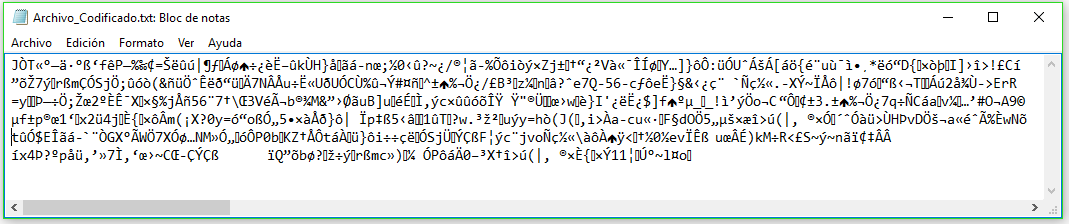
\includegraphics[width=1\textwidth, right]{./imagenes/prog1.png}\\
		Figura 1.-Texto codificado.
	\end{center}
En la Figura 1 podemos ver la salida tras la ejecucion del programa, el cual nos arrojara un archivo codificado.

	\begin{center}
		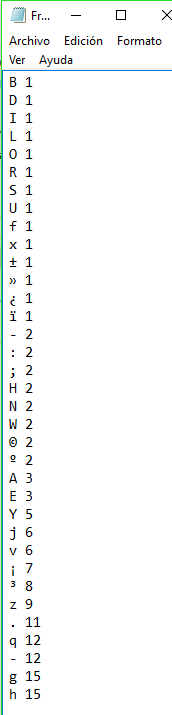
\includegraphics[scale=.5]{./imagenes/prog2.png}\\
		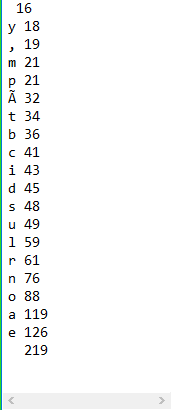
\includegraphics[scale=.5]{./imagenes/prog3.png}\\
		Figura 2.-Tabla de frecuencias.
	\end{center}
En la Figura 2 podemos ver la tabla de frecuencias de los distintos caracteres en el archivo.

	\begin{center}
		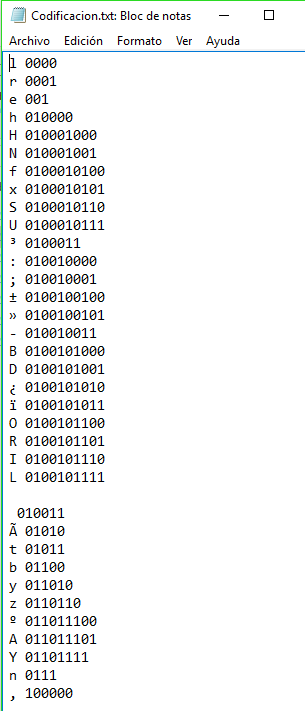
\includegraphics[scale=.5]{./imagenes/prog4.png}\\
		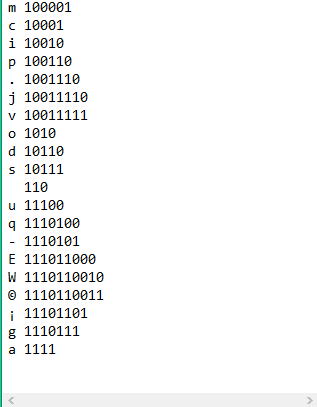
\includegraphics[scale=.5]{./imagenes/prog5.png}\\
		Figura 3.-Tabla de frecuencias.
	\end{center}
En la Figura 3 podemos ver la codificacion que le corresponde a cada caracter del archivo original.
\newpage
	\begin{center}
		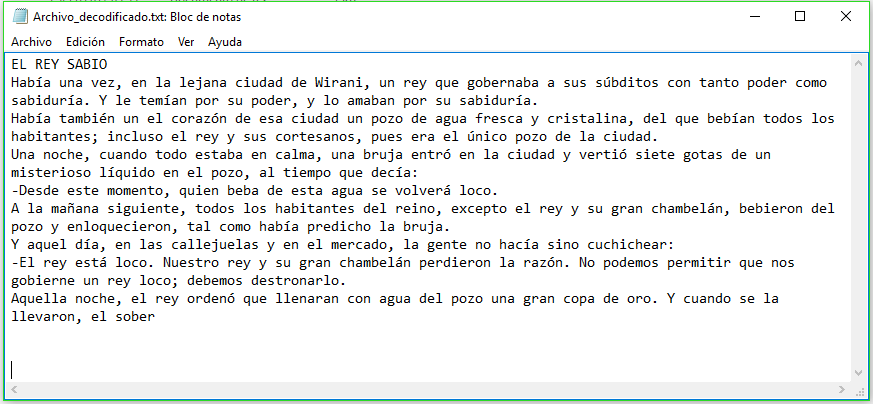
\includegraphics[scale=.5]{./imagenes/prog6.png}\\
		Figura 4.- Archivo Decodificado
	\end{center}
En la Figura 4 se observa el archivo decodificado.\\Aquí tengo un error, no se porque motivo no me esta decodificando todo el documento, pero se alcanza a ver parte de este. Y, hasta donde lo hace, lo va haciendo bien.

\begin{center}
		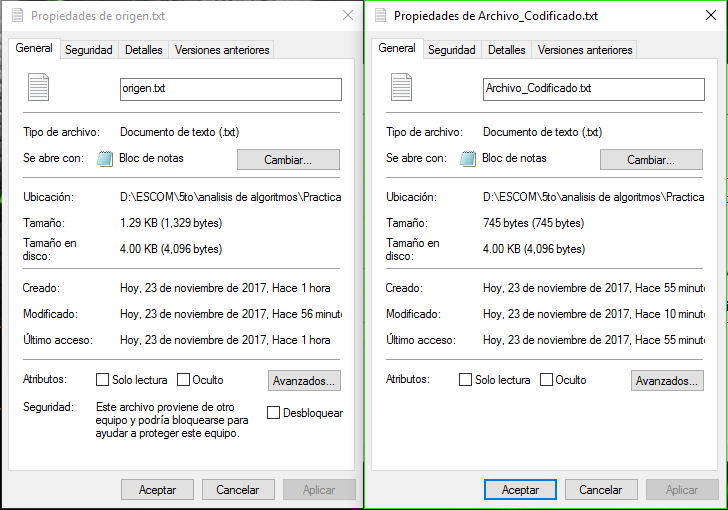
\includegraphics[scale=.5]{./imagenes/prog7.png}\\
		Figura 5.- Archivo Decodificado
	\end{center}
En la Figura 5 podemos ver la comparacion de tamaños de archivos, siendo el izquierdo el Original, y el derecho el Codificado, podemos ver que el archivo codificado pesa menos.\\Esto se lo podria tribuir a que el archivo se corta en algun punto. Aunque estoy seguro que la dcodificacion si bajo el peso del documento.

	\newpage

	\section{Conclusi\'on}
Fue muy interesante ver el comportamiento del algoritmo de Huffman, ver como va tomando secuerncias y las utiliza para comprimir un texto es algo muy interesante, se me ocurre que, ya que de igual modo llevo Cryptography, se podria combinar con algun modo de operacion del AES o del DES, y dar lugar a algo interesante de analizar en ambas clases.\\Tuve algunos problemas que sinceramente no pude resolver, ya que no supe porque , al momento de decodificar el archivop no me daba el archivo oiginal, y se quedaba a medias.\\Fue una de las practicas mas complicadas que hemos hecho, o almenos a mi parecer, asi fue.
	

	\bigskip

	\newpage

	\section{Bibliografía}
	\begin{itemize}
		\item Brassard, G. (1997). Fundamentos de Algoritmia. España: Ed. Prentice Hall. ISBN 		848966000X
		\item Harel, D. (2004). Algorithmics: The spirit of Computing (3rd. Ed). Estados Unidos de América: Addison
Wesley. ISBN-13: 978-0321117847
	\end{itemize}


\end{document}